\begin{itemize}
\item All the data can be tabularised as:

\begin{table}[!ht]
\centering
\resizebox{\columnwidth}{!}{\begin{tabular}{|c|c|c|c|} 
\hline
 & Grinding machine&Sprayer&Profit\\
\hline
\textbf{Pedestal lamps} & 2 & 3 & 5 \\ 
\hline
\textbf{Wooden shades} & 1  & 2 & 3 \\ 
\hline
\text{Max Hours} & $\leq12$&$\leq20$&\\
\hline
\end{tabular}}
\caption{Time needed and Profit for each object}
\label{opt/17/tab:table1}
\end{table}
\item Let the number of pieces of pedestal lamp manufactured be $x$ and
the number of pieces of wooden shades manufactured be $y$ such that : 
\begin{align}
    x \geq 0 
    \\
    y \geq 0 
\end{align}
\item From the data given we have:
\begin{align}
    2x+y &\leq 12 
\end{align}
and,
\begin{align}
    3x+2y &\leq  20
\end{align}
$\therefore$ The maximizing function is:
\begin{align}
        \max Z &= \myvec{5& 3}\vec{x}\\
        s.t. \quad 
        \myvec{2 & 1\\ 3 & 2 }\vec{x} &\preceq \myvec{12\\20} \\
        \vec{-x} &\preceq \vec{0}
\end{align}
\item The Lagrangian function can be given as:
\begin{equation}
\begin{aligned}
    &L(\vec{x},\boldsymbol{\lambda}) \\ &= \myvec{5 & 3}\vec{x}+\lcbrak{\sbrak{\myvec{2 & 1}\vec{x}-12}} \\ &+ \sbrak{\myvec{3 & 2}\vec{x}-20} \\ &+ \sbrak{\myvec{-1 & 0}\vec{x}} +\rcbrak{\sbrak{\myvec{0 & -1}\vec{x}}}\boldsymbol{\lambda}
\end{aligned}
\end{equation}
where,
\begin{align}
    \boldsymbol{\lambda} &= \myvec{\lambda_1 \\ \lambda_2 \\ \lambda_3 \\ \lambda_4}
\end{align}
\item Now, we have
\begin{align}
    \nabla L(\vec{x},\boldsymbol{\lambda}) &= \myvec{5 + \myvec{2 & 3 & -1 & 0 }\boldsymbol{\lambda}\\ 3 +\myvec{1 & 2 &0 & -1}\boldsymbol{\lambda} \\ \myvec{2 & 1}\vec{x}-12 \\ \myvec{3 & 2}\vec{x}-20 \\ \myvec{-1 & 0}\vec{x} \\ \myvec{0 & -1}\vec{x}}
\end{align}
$\therefore$ The Lagrangian matrix is given by:-
\begin{align}
  \small{\myvec{0 & 0 & 2 & 3 & -1 & 0 \\ 0 & 0 & 1 & 2 &0 & -1 \\ 2 & 1 & 0 & 0 & 0 & 0 \\ 3 & 2 & 0 & 0 & 0 & 0 \\ -1 & 0 & 0 & 0 & 0 & 0 \\ 0 & -1 & 0 & 0 & 0 & 0 }\myvec{\vec{x} \\ \boldsymbol{\lambda} }}= \small{\myvec{-5 \\ -3 \\ 12 \\ 20 \\ 0 \\0 }}
\end{align}
\item Considering $\lambda_1,\lambda_2$ as only active multiplier,
\begin{align}
    \myvec{0 & 0 & 2 & 3  \\ 0 & 0 & 1 & 2 \\ 2 & 1 & 0 & 0 \\3 & 2 & 0 & 0}\myvec{\vec{x}\\ \boldsymbol{\lambda}} &= \myvec{-5 \\ -3 \\ 12 \\ 20}
\end{align}
\begin{align}
 \implies   \myvec{\vec{x} \\ \boldsymbol{\lambda}} &=  \myvec{0 & 0 & 2 & 3  \\ 0 & 0 & 1 & 2 \\ 2 & 1 & 0 & 0 \\3 & 2 & 0 & 0} ^{-1}\myvec{-5 \\ -3 \\ 12 \\ 20}
    \\
    \implies   \myvec{\vec{x} \\ \boldsymbol{\lambda}} &= \myvec{0 & 0 & 2 & -1 \\ 0 & 0 & -3 & 2 \\ 2 & -3 & 0 & 0 \\ -1 & 2 & 0 & 0}\myvec{-5 \\ -3 \\ 12 \\ 20}
    \\
    \implies \myvec{\vec{x} \\ \boldsymbol{\lambda}} &= \myvec{4\\24 \\ -1 \\ -1 }
\end{align}
$\because \boldsymbol{\lambda}=\myvec{-1 \\ -1} \prec \vec{0}$
\\
\item The Optimal solution is given by:
\begin{align}
    \vec{x} &= \myvec{4\\4} \\
    Z &= \myvec{5&3}\vec{x} \\
   Z &= \myvec{5&3}\myvec{4 \\ 4} \\
    Z&= \text{Rs.} 32
\end{align}
\item So, to maximise profit
\\
 No. of pedestal lamps manufactured is \boxed{x=4} and
 
 No. of wooden shades manufactured is \boxed{y=4}.  This is verified in Fig. \ref{opt/fig/17}
\item The maximum daily profit is \boxed{Z=\text{Rs.} 32} .
%
\begin{figure}[!ht]
\centering
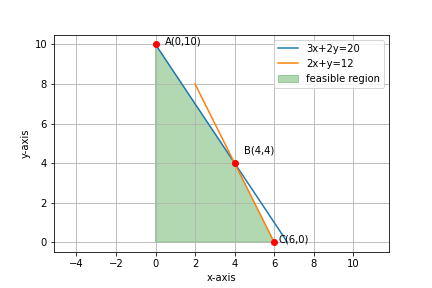
\includegraphics[width=\columnwidth]{solutions/su2021/2/17/assignment11.png}
\caption{Graphical Representataion}
\label{opt/fig/17}
\end{figure}
\end{itemize}

